\documentclass[aspectratio=169]{beamer}

\let\val\undefined
\usepackage{pgf}
\usepackage{pgfplots}
\usepackage{tikz}
\usepackage{booktabs}
\usepackage{natbib}
\usepackage{framed}
\usepackage{longtable}
\usepackage{bigdelim,multirow}
\usepackage{amsmath}
\usepackage{amsthm}
\usepackage{mathtools}
\pgfplotsset{compat=1.15} 
\usepackage{algorithmic}

\usetikzlibrary{arrows,automata,backgrounds,positioning,decorations,intersections,matrix}

% *** Styles ***
\setbeamertemplate{navigation symbols}{}
\usecolortheme{dolphin}
%\usecolortheme{rose}
\setbeamercovered{transparent}
\usefonttheme{professionalfonts}
%\usefonttheme[onlymath]{serif}

% 
\addtobeamertemplate{navigation symbols}{}{%
    \usebeamerfont{footline} %
    \usebeamercolor[fg]{footline}%
    \hspace{1em}%
    \insertframenumber/\inserttotalframenumber
}

\DeclarePairedDelimiter{\norm}{\lVert}{\rVert}
\DeclarePairedDelimiter\abs{\lvert}{\rvert}%


% \setlist[itemize,1]{label=$\times$}
% \setlist[itemize,2]{label=$\checkmark$}
% \setlist[itemize,3]{label=$\diamond$}
% \setlist[itemize,4]{label=$\bullet$}


% *** Colors ***
\newcommand{\tc}[2]{\textcolor{#1}{#2}}
\newcommand{\tcb}[1]{\tc{blue}{#1}}
\newcommand{\tcr}[1]{\tc{red}{#1}}
\newcommand{\tcg}[1]{\tc{green}{#1}}

\def\checkmark{\tikz\fill[scale=0.4](0,.35) -- (.25,0) -- (1,.7) -- (.25,.15) -- cycle;} 

\newcommand{\Ex}{\mathbb{E}}
%\newcommand{\Pr}{\mathbb{P}}
\DeclareMathOperator{\Var}{Var}

\definecolor{varcolor}{RGB}{132,23,49}
\newcommand{\varname}[1]{\textcolor{varcolor}{\mathsf{#1}}}

\title{Learning safe policies with expert guidance \\
{\footnotesize Jessie Huang, Fa Wu, Doina Precup, Yang Cai}\\
{\footnotesize McGill University} \\
{\footnotesize NIPS 2018} }
\date{}

\begin{document}
\begin{frame}
	\maketitle

\end{frame}
%=====================================%
\begin{frame}
	\frametitle{Problem Definition}
	\begin{itemize}
		\item Given:
			\begin{itemize}
				\item demonstrations from expert
			\end{itemize}
		\item Asked:
			\begin{itemize}
				\item safe policy
			\end{itemize}
		\item Method:
			\begin{itemize}
				\item ellipsoid based optimization
			\end{itemize}
		\item Assumption:
			\begin{itemize}
				\item $R(s) = w.\phi(s)$, where $\phi(s)$ is a vector of features
			\end{itemize}
		\item Value Funciton:

				$$
				\begin{matrix*}[l]
					\mathbb{E}_{s_0 \sim D}[V^\pi (s_0) | M] & = \mathbb{E}[\sum_{t=0}^{\infty}\gamma^t w.\phi(s_t) | \pi] \\
					 & = w.\mathbb{E}[\sum_{t=0}^{\infty}\gamma^t \phi(s_t) | \pi] \\
					 & = w. \Psi(\pi)
				\end{matrix*}
				$$
	\end{itemize}

	
\end{frame}
%=====================================%
%=====================================%

\begin{frame}
	\frametitle{Background}
	\begin{itemize}
		\item Robust MDP:
		\begin{itemize}
			\item Which policy gives us the most in the worst condition?
			\item Maxmin learning
			\[
				\max_{\mu \in P_F} \min_{w \in P_R} \mu^\top w 
			\]
			\item By strong duality
			\[
				\begin{matrix*}[l]
					\max & z \\
					s.t. & z \leq \mu^\top w, \quad \forall w \in P_R \\
					 	 & \mu \in P_F
				\end{matrix*}
			\]
		\end{itemize}
	\end{itemize}
\end{frame}
%=====================================%
%=====================================%

\begin{frame}
	\frametitle{Background}
	\begin{itemize}
		\item Problem?
			\begin{itemize}
				\item Coming up with a reasonable $P_F$
				\item Too many possible rewards $w \in P_R$
			\end{itemize}
		\item Idea?
			\begin{itemize}
				\item Every Linear Program can be turned into a series of feasibility problem
			\end{itemize}
		\item How?
			\begin{itemize}
				\item
				\[
					\begin{matrix*}[r]
						\max \quad c^\top x & & c^\top x \geq c_0\\
						Ax \leq b & \equiv & Ax \leq b\\
						x \geq 0 & &x \geq 0 
					\end{matrix*}
				\]
				% \begin{algorithmic}
				% 	\STATE initialize $c_0$
				% 	\IF {I is feasible}
				% 	\STATE $c_0 \gets c_0/2 $
				% 	\ELSE
				% 		\RETURN $c_0$
				% 	\ENDIF
				% \end{algorithmic}

				% Example

				% \begin{algorithmic}
				% \STATE $i\gets 10$
				% \IF {$i\geq 5$} 
				%         \STATE $i\gets i-1$
				% \ELSE
				%         \IF {$i\leq 3$}
				%                 \STATE $i\gets i+2$
				%         \ENDIF
				% \ENDIF 
				% \end{algorithmic}
				\item if feasible, the optimum is smaller than $c_0$. So, we decrease $c_0$ by a factor of 2
				\item if not feasible, the optimum is in the interval of $[c_0/2, c_0]$
				\item initial $c_0$ should be sufficiently large 
			\end{itemize}
	\end{itemize}
\end{frame}
%=====================================%
%=====================================%

\begin{frame}
	\frametitle{Optimization vs. Feasiblity}
	\begin{itemize}
		\item It turns into a binary search
		\item Solves in polynomial time in the input size
		\item An intuitive way of addressing feasibility problem is called \tcg{Ellipsoid Algorithm}
	\end{itemize}

	\begin{figure}
		\centering
		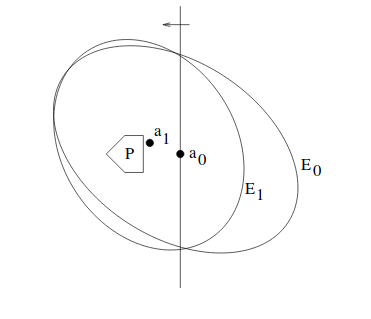
\includegraphics[scale=.40]{ellips.png}
		% \caption{Ellipsoid Algorithm}
		\label{ellipsoid}
	\end{figure}

\end{frame}
%=====================================%
%=====================================%

\begin{frame}
	\frametitle{Ellipsoid Algorithm}
	\begin{figure}
		\centering
		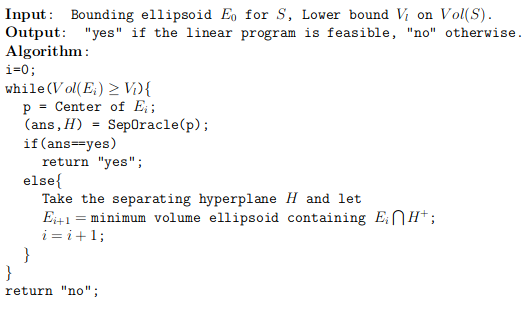
\includegraphics[scale=.60]{alg.png}
	\end{figure}
\end{frame}
%=====================================%
%=====================================%

\begin{frame}
	\frametitle{Separation Oracle}
	\begin{figure}
		\centering
		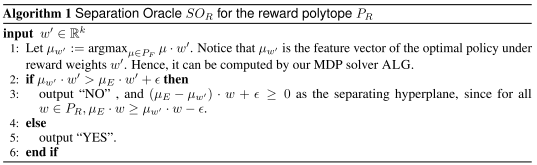
\includegraphics[scale=.60]{so.png}
	\end{figure}
\end{frame}
%=====================================%
%=====================================%

\begin{frame}
	\frametitle{Separation Oracle}
	\begin{figure}
		\centering
		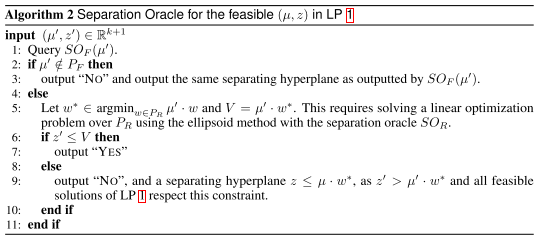
\includegraphics[scale=.60]{somain.png}
	\end{figure}
\end{frame}
%=====================================%
%=====================================%

\begin{frame}
	\frametitle{A problem, and a solution!}
	\begin{itemize}
		\item Problem:
		\begin{itemize}
			\item Despite the mathematical proof of polynomial time complexity, it does worse than simplex
		\end{itemize}
		\item Solution:
		\begin{itemize}
			\item Using follow-the-pertubed-leader
		\end{itemize}
	\end{itemize}
\end{frame}
%=====================================%

%=====================================%

\begin{frame}
	\begin{center}
		\Huge Thank You!
	\end{center}
\end{frame}
%=====================================%

% \begin{frame}
	% \frametitle{Background}
% 	\begin{itemize}
% 		\item 
% 	\end{itemize}
% \end{frame}


\end{document}
